%==============================================================================
% experiments.tex — Experimental Setup for PP-HFM
% Self-contained \section{}; \input this into main.tex (never compile alone).
%
% Structured after the house experimental-setup template: Datasets,
% Implementation Details, Evaluation Metrics (defined as numbered equations),
% Experimental Protocol, closing with a forward pointer to Results.
%
% Equation numbering CONTINUES from method.tex, which ends at (15).
%
% Every figure here is established fact verified against an artifact:
%   partition_meta.json   client counts, edge map, split sizes, class balance
%   datasets.py registry  channel counts, modality contracts, pairing
%   labels.npy            outcome prevalence
%   installed packages    library versions
% No measured outcome appears in this section; outcomes are in Section V.
% READABILITY PASS 2026-10-21: formal register; equations/figure verbatim.
%==============================================================================

\section{Experimental Setup}
\label{sec:experiments}

Fig.~\ref{fig:workflow} outlines the study from partitioning to audit.

\begin{figure*}[!t]
\centering
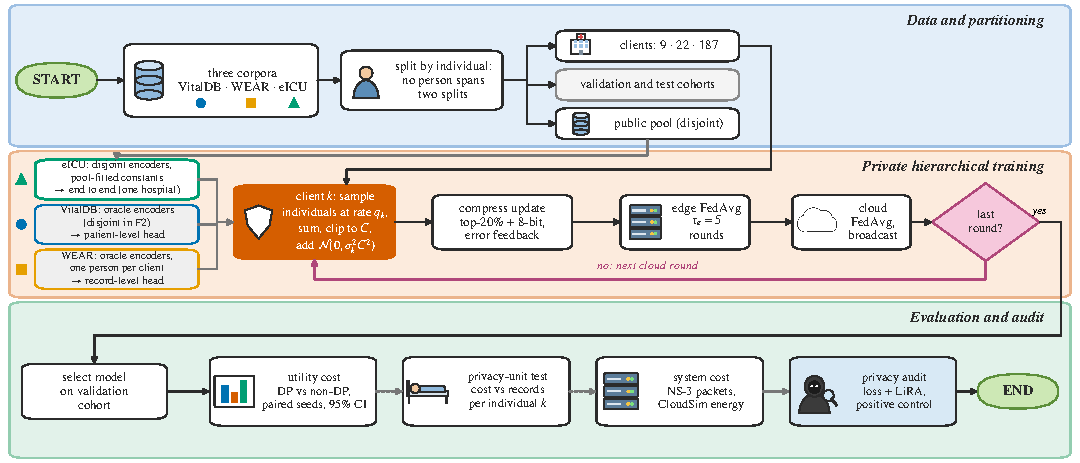
\includegraphics[width=\textwidth]{fig00_workflow.pdf}
\caption{Study workflow: individual-level partitioning, per-corpus encoder
configuration (end to end on eICU only, for individuals at one hospital), private hierarchical training and
paired evaluation with an attack audit.}
\label{fig:workflow}
\end{figure*}

\subsection{Datasets}

The framework is evaluated on two publicly available multimodal corpora:
VitalDB \cite{ref20}, a clinical monitoring collection of non-cardiac surgical
cases, and WEAR \cite{ref21}, an outdoor activity collection combining
body-worn inertial sensing with egocentric video. A third corpus, the eICU
Collaborative Research Database \cite{ref27}, distributed through PhysioNet
\cite{ref28} under a credentialed data-use agreement, serves as an external
clinical corpus. In all three corpora, the two modalities originate from the
same individual and are paired at the source rather than by a construction
rule. This
property is necessary for a claim about fusion, since a fusion benefit under
rule-based pairing may reflect the rule rather than complementary information.
The corpora also cover the two deployment regimes relevant to the privacy
mechanism: a client holding many individuals and a client holding one.

In VitalDB, modality~A is the intraoperative monitoring record with eighteen
channels, namely nine numeric physiological trends and nine binary indicators
of whether each trend was recorded. Modality~B is a thirty-four-dimensional
vector of preoperative clinical and laboratory variables. All channels of a
case originate from the same patient during the same operation and are
time-aligned at capture across the waveform digitizer, the patient monitor and
the anesthesia machine. The prediction target is postoperative admission to
intensive care, which is positive in $18.84\,\%$ of windows ($19.65\,\%$ in
the case-level partition defined below). In WEAR,
modality~A consists of twelve inertial channels and modality~B is a
$2048$-dimensional two-stream video feature computed over the same interval and
synchronized in hardware. The task is activity recognition over eighteen
classes.

In eICU, modality~A consists of twelve channels: six vital signs recorded
during the ICU stay (heart rate, respiratory rate, oxygen saturation, systolic
and diastolic arterial pressure, and temperature) and six binary indicators of
whether each was observed. The first $24$ hours after unit admission are
divided into non-overlapping $60$-minute windows of twelve $5$-minute slots,
and a window is retained only if at least three slots are observed.
Modality~B is a five-dimensional vector recorded at or before admission (age,
sex, admission weight, admission height and the APACHE score) for the same
stay. The prediction target is in-unit mortality, with a prevalence of
$0.0422$. Individuals who die within the observation window are excluded,
since their final windows are peri-mortem and pose no prediction problem.
Prediction is therefore made at hour $24$, when the APACHE score, computed
from the worst values of the first day, is available. The
resulting corpus contains $3{,}782{,}805$ windows from $185{,}140$ stays of
$132{,}736$ individuals.

Each corpus is partitioned into disjoint training, validation and test
subsets, which are fixed across all experiments, so no record appears in more
than one subset and all arms use the same split. VitalDB is evaluated on two
partitions, both distributing cases across nine clients by surgical specialty
and two edge aggregators. The \emph{person-level} partition assigns each
person to one split and one client; cases that would place a person in a
second split or on a second client are removed ($200$ cases). It contains
$33{,}491$ training, $6{,}773$ validation and $6{,}895$ test windows from
$4{,}221$, $868$ and $885$ persons, with $7.9$ training windows per
individual on average. The \emph{case-level} partition of the earlier
experiments splits by operation ($34{,}044$, $7{,}308$ and $7{,}360$ windows
from $6{,}257$ operations); in it, $55$ of $940$ test persons also have a
training case and $68$ training persons span two clients, so its results
protect the operation rather than the person. The privacy cost, the cost of
the unit and the comparison with prior systems are person-level; all other
VitalDB results are case-level and marked as such. No test case of either
partition was used to pretrain the encoders. For WEAR, the partition contains $26{,}424$ training,
$5{,}395$ validation and $5{,}969$ test windows across twenty-two clients, one
per participant, also assigned to two edges. Partitioning by specialty rather
than at random produces realistic heterogeneity, since specialties differ in
case mix, outcome prevalence and routinely recorded channels
(Fig.~\ref{fig:noniid}). For eICU, the clients are the hospitals themselves,
taken as given rather than constructed. Of $206$ hospitals, those with fewer
than $200$ windows or with no positive outcome are pooled into a single
client, giving $187$ clients assigned to two edge aggregators, with a median of
$444$ individuals per client and $28.50$ records per individual. Splits are
made by individual, stratified by outcome within each client, because an
individual may be admitted more than once, and a stay-level split would place
the same person in both training and test data. Case-level metrics on eICU are
grouped by stay rather than by individual, because the outcome of a person can
differ between admissions. The validation subset is used only for model
selection, and the test subset only for final evaluation.

\begin{figure*}[!t]
\centering
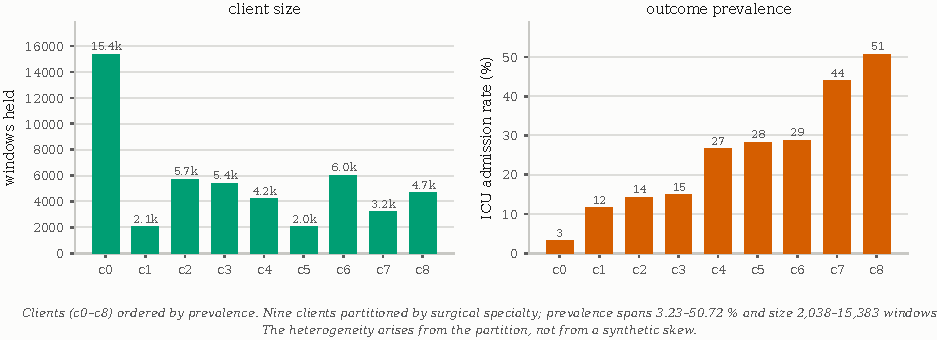
\includegraphics[width=\textwidth]{fig6_noniid.pdf}
\caption{Heterogeneity of the clinical partition (case-level). Partitioning by surgical
specialty rather than at random yields clients that differ by a factor of
seven in size and by more than fifteen in outcome prevalence, from $3.23\,\%$
to $50.72\,\%$. The skew is a property of how care is organized, not an
artifact imposed for the experiment.}
\label{fig:noniid}
\end{figure*}

Four controls are applied in preparing the clinical corpus, each preventing an
inflation of the reported results that would not be visible during training.
First, data are split by case, so all windows of an operation fall in the same
subset; a window-level split would place highly correlated near-duplicates of
training examples in the test set. Second, modality~B is restricted to
preoperative variables, and all intraoperative columns are excluded, because
interventions such as transfusion or vasopressor administration are given in
response to deterioration and therefore encode the outcome. Third, missing
values are not simply imputed: gaps are filled within a case and paired with
an explicit binary indicator, because, for example, an arterial line is placed
only in patients judged to be at risk, so its absence carries information
about acuity. Fourth, normalization statistics are computed over training cases
only, with estimators that handle missing values, because a naive estimator
returns an undefined statistic for a fully missing channel and propagates it to
every window. In addition, a separate set of individuals, disjoint at the
individual level from all client data, is reserved before federated training
and used only to pretrain the encoders, so that the reported budget holds end
to end. For eICU, this pool contains $526{,}867$ windows, leaving
$2{,}122{,}350$ training, $563{,}948$ validation and $569{,}640$ test windows
for the clients.

\subsection{Implementation Details}
\label{sec:exp:impl}

All arms use the same training configuration, so that differences can be
attributed to the mechanism under test. Each client performs one local pass per
federated call, five edge rounds are executed per cloud round, and training
runs for ten cloud rounds. The privatized gradient is passed to Adam
(learning rate $10^{-3}$, weight decay $10^{-4}$), which is post-processing,
with a per-individual clipping norm of one, $64$
individuals sampled per step in expectation, and a noise multiplier per client
from the calibration of \eqref{eq:6}.
Updates are sparsified to the largest twenty percent of coordinates and
quantized to eight bits before transmission, with error feedback of the
residual. The full budget goes to training: $\varepsilon = 0.9$ on the
clinical deployments. The encoders are pretrained centrally and then frozen, so the
privatized parameters are those of the fusion head only: $559{,}874$ of
$1{,}864{,}227$ parameters, or $30.0\,\%$.

Unless stated otherwise, all results, including the system-level objectives,
the privacy--utility comparisons and the membership-inference audit, were
obtained with the \emph{oracle} encoder configuration of
Section~\ref{sec:method:backbone}, in which the encoders were pretrained on the
pooled client training data. This configuration does not provide a valid
end-to-end guarantee. It is used because it isolates the behavior of the
privatized head from the origin of the representation, and because using the
same encoders in every arm keeps the comparisons between arms controlled. The
\emph{disjoint} configuration, which provides the guarantee, is evaluated
separately, and the difference is reported in
Section~\ref{sec:results:objectives} as the cost of a valid guarantee. On eICU,
every experiment that uses pretrained encoders uses the disjoint
configuration.
Absolute utilities should therefore be read as upper bounds for the deployable
configuration, whereas differences between arms, on which the claims rely, are
unaffected. All normalization layers are group or layer normalizations, as
explained in Section~\ref{sec:method:backbone}.

Models are implemented in PyTorch~2.5, with per-sample gradients and R\'enyi
accounting provided by Opacus~1.5. Deployment models are exported to ONNX at
full precision, and inference is timed with ONNX Runtime on the CPU
provider of a workstation (Intel Core i7-14700), since an edge node cannot be
assumed to have an accelerator; no edge hardware was used. Network behavior is simulated in ns-3~3.46,
with the device-to-edge segment over a wireless local-area link and the
edge-to-cloud segment over a point-to-point backhaul. Energy is modeled in
CloudSim~Plus separately for the device, edge and cloud tiers. Training was
performed on a single workstation with one NVIDIA RTX~A2000 GPU.
Table~\ref{tab:params} collects these parameters.

\begin{table}[!t]
\centering
\caption{Training and evaluation parameters}
\label{tab:params}
\footnotesize
\setlength{\tabcolsep}{4pt}
\begin{tabular}{@{}p{0.40\columnwidth}p{0.56\columnwidth}@{}}
\toprule
Parameter & Value \\
\midrule
Cloud rounds $R$; edge rounds $\tau_e$ & $10$; $5$ \\
Edge aggregators $E$ & $2$ (eICU scaling test: $2$--$16$) \\
Local passes per edge round & $1$ \\
Optimizer & Adam \\
Learning rate; weight decay & $10^{-3}$; $10^{-4}$ \\
Expected individuals per step $B$ & $64$ \\
Clipping norm $C$ & $1$ \\
Training budget & $\varepsilon = 0.9$, $\delta = 10^{-5}$ \\
Accountant & privacy loss distribution, per-client $\sigma_k$ \\
Records per patient (cap) & $64$ \\
Update encoding & top-$20\,\%$, $8$-bit, error feedback \\
Seeds & $5$ (paired); $3$ for grids \\
LiRA shadow models & $16$ \\
Latency timing & P95, $1{,}000$ runs, $100$ warm-up \\
Software & PyTorch~2.5, Opacus~1.5, ONNX Runtime, ns-3~3.46, CloudSim~Plus~8.5 \\
Hardware & one NVIDIA RTX~A2000 GPU \\
\bottomrule
\end{tabular}
\end{table}

\subsection{Evaluation Metrics}

Classification performance is assessed with two complementary measures. The
area under the receiver operating characteristic curve summarizes ranking
performance across all decision thresholds. Average precision summarizes the
precision--recall trade-off,
%
\begin{equation}
\mathrm{AP} = \sum_{n} \big(R_n - R_{n-1}\big)\, P_n,
\tag{14}
\label{eq:16}
\end{equation}
%
where $P_n$ and $R_n$ are the precision and recall at the $n$th threshold.
Average precision is reported because the clinical task is imbalanced, with
$18.84\,\%$ positive windows. Under this imbalance, accuracy is nearly
uninformative, since a constant negative prediction achieves about four-fifths
accuracy, and the area under the ROC curve is optimistic. Average precision
reflects performance on the minority class.

Metrics are also aggregated per individual. The model scores windows, but the
clinical question concerns an operation, and windows of the same case are
highly correlated, so window-level metrics overstate the effective sample size.
The predictions of a case are therefore averaged,
%
\begin{equation}
\bar{p}_c = \frac{1}{|W_c|} \sum_{w \in W_c} p_w ,
\tag{15}
\label{eq:17}
\end{equation}
%
giving one prediction per individual. Case-level metrics are computed from
$\bar{p}_c$ using the same expressions as for $p_w$.

Comparisons between arms are paired by seed, since the arms share their
partition, initialization schedule and calibration data. For $S$ paired seeds
with per-seed difference $d_s$, the reported interval is
%
\begin{equation}
\bar{d} \pm t_{S-1,\,0.975}\, \frac{s_d}{\sqrt{S}},
\tag{16}
\label{eq:18}
\end{equation}
%
where $s_d$ is the sample standard deviation of the differences. Student's $t$
distribution is used instead of a normal approximation because the number of
seeds is small. Seed counts are fixed before each comparison and are not
increased after inspecting the results.

Communication, latency, reliability and energy are reported as defined in
Section~\ref{sec:method:instr}, and every network quantity is measured on
rounds in which the payload traversed the simulated topology.

\subsection{Experimental Protocol}

The proposed system is compared with differentially private federated
averaging in three configurations, each isolating one design decision. The
first trains the full parameter vector under the privacy budget, which is the
conventional application of DP-SGD to a federated model. The second restricts
private optimization to the fusion head over randomly initialized frozen
encoders, isolating the effect of reducing the privatized dimension. The third
restricts private optimization to the fusion head over \emph{pretrained} frozen
encoders. This arm controls for a confound: without it, the benefit of
parameter-efficient private training cannot be separated from the benefit of
the pretrained representation. A non-private model trained with an otherwise
identical recipe provides the reference for the accuracy cost of the budget.
All arms share the partition, schedule, compression settings and evaluation
procedure, and differ only in the factor under test.

The same evaluation protocol is applied to every arm. The checkpoint with the
highest validation performance is retained, without use of test data. Each
retained checkpoint is evaluated once on the test subset, and all metrics are
computed from the same predictions with the same aggregation.

The privacy guarantee is audited by individual-level membership inference
using the two attacks of Section~\ref{sec:method:mia}. Each attack is also
applied to a configuration known to memorize, namely non-private training of
the same head over the same frozen encoders, as a positive control. A negative
result is accepted only if the same procedure detects clearly elevated leakage
on the control.

A further experiment separates the two sources of the cost of the
individual-level unit. Moving the guarantee from the record to the individual
both reduces the number of units sampled per step and bounds the summed
contribution of each individual, and the aggregate comparison cannot separate
the two. The number of units sampled per step is therefore held equal in both
arms, which removes the first effect and leaves only the clipping geometry,
and the number of training records retained per patient, $k$, is varied over
$\{1, 2, 4, 8\}$ with three seeds at $\varepsilon = 1$. Subsampling is applied
to the training partition only; validation and test sets are unchanged, so
every configuration is evaluated on the same held-out data. Because reducing
$k$ also reduces the training set size, absolute utility decreases with $k$ and
is not comparable across $k$. The quantity of interest is the paired difference
between arms at each $k$, where both arms use the same data, partition and
seed. At $k = 1$, a patient contributes a single record, so the two arms must
agree, which provides a falsification test of the design.
